\documentclass[11pt]{article}
\linespread{1.5}

\usepackage{preamble}
\usepackage[spanish,es-tabla]{babel}


\begin{document}

\pagenumbering{gobble}
{

% Title
\subfile{title}

% Abstract
% \subfile{abstract}

\newpage

\hypersetup{linkcolor=black}

\renewcommand\contentsname{Índice de contenido}
\tableofcontents

\clearpage

% List of codes
\tcblistof[\section*]{code}{Índice de código}
% List of theorems
% \tcblistof[\section*]{theorem}{\theoListTitle}
% List of figures
\renewcommand\listfigurename{Índice de figuras}
\listoffigures
% List of tables
\renewcommand\listtablename{Índice de tablas}
\listoftables

}
\clearpage
\pagenumbering{arabic}

% ACRONYMS
\printglossary[type=\acronymtype, title=Glosario de acrónimos, nonumberlist]\ \label{sec:acronyms}

% ------------------------- CONTENT ------------------------- %

\section{Introducción}

Las micotoxinas son toxinas naturales derivadas del metabolismo secundario de mohos micotoxigénicos, que se pueden encontrar en alimentos y materias primas. Una de ellas,
el \acrfull{don}, se encuentra en el campo predominantemente en granos de cereales como el trigo. Por este motivo, el deoxinivalenol se encuentra frecuentemente en
alimentos a base de cereales lo que, unido a la elevada ingesta de trigo típica de la dieta española, hace que la exposición de la población sea significativa. En los años
en que la meteorología es especialmente adversa los cultivos de todo el mundo muestran altos niveles de contaminación. Además, en los últimos años existe una creciente
evidencia de un aumento en la incidencia de micotoxinas como resultado del cambio climático.

Actualmente, las empresas procesadoras de cereales basan su autocontrol en el análisis de muestras de un determinado número de lotes mediante técnicas inmunocromatográficas
rápidas, de forma que se rechazan los lotes no conformes. Los lotes que, una vez analizados, superan el límite legal \(1250 \mu g/kg\), en general, se desvían íntegramente
a la alimentación animal. En el sector de la alimentación animal, el problema se hace más evidente, ya que el consumo de piensos contaminados se evidencia en una menor
ganancia de peso del ganado y el impacto en otros parámetros productivos y de salud animal.


\subsection{Motivación}

El desafío que se plantea se centra en las operaciones de selección y clasificación de granos mediante \acrfull{nir-hsi}, previas a la transformación, que
de ser efectivas podrían aplicarse a lotes que superen los \(1250 \mu g/kg\), con la intención de devolver dichos lotes a la cadena alimentaria, una vez se ha separado
la fracción más contaminada. De esta manera, la fracción que podría destinarse al consumo humano sería posiblemente mayoritaria, y el sistema de producción de alimentos,
en su conjunto, más sostenible. Como consecuencia, las motivaciones son las contribuciones a la seguridad alimentaria y ambiental con protección a través de nuevas 
tecnologías que permitan aplicaciones avanzadas para la agricultura y los sistemas alimentarios, a evitar pérdidas y derroche alimentario; pues los métodos actuales de 
control de calidad no permiten un control óptimo. La inspección por \gls{nir-hsi} puede permitir superar este problema.


\subsection{Objetivos}

Nuestro objetivo como parte del proyecto es claro, construir un modelo de predicción robusto con los datos que tenemos, la validación de los modelos generados y la técnica en
condiciones de laboratorio con un número suficiente de muestras reales y el desarrollo de software para la detección en tiempo real de granos contaminados. 

Para ello, hemos separado esta tarea en diferentes pasos discernibles. 

\begin{enumerate}
    \item Entender los datos de los resultados de laboratorio.
    \item Entender el existente proceso de análisis de imágenes hiperespectrales.
    \item Tratar de mejorar el actual proceso de análisis de las imágenes.
    \item Entender el actual proceso de entranamiento y análisis de modelos de \gls{ml}.
    \item Tratar de mejorar el preprocesado de los datos, tanto como el entrenamiento de nuevos modelos para tratar de obtener mejores resultados.
    \item Entrenar buenos modelos de \gls{ml} que, según las imágenes hiperespectrales, sean capaces de predecir si un grano está contaminado. 
    \item Una vez entrenados los modelos básicos, tratar de ajustarlos a los datos con \textit{Hyperparameter tuning}.
    \item Añadir nuevos modos de ejecución del programa para emular la carga continua de imágenes que habría en un caso de uso real, además de prepararlo para que se 
    pueda ejecutar por un tiempo indefinido como en un caso real, guardando los resultados de las predicciones.
\end{enumerate}

\subsection{Estructura del documento}


\section{Análisis del problema}

El principal problema que nos concierne es la detección y separación del grano contaminado de la corriente de cereal circulando por los transportadores. Para solucionarlo,
la propuesta de sistema a implementar consiste en la instalación de cámaras infrarojas en la línea de procesado, capaces de captar las imágenes hiperespectrales de la
corriente. De manera que utilizando nuestro modelo previamente calibrado, se detecte cuáles son los granos más contaminados y se puedan separar por una corriente de aire. 
Podemos ver un esquema del sistema en la \textit{imagen\ \ref{fig:detection-system}}.

\begin{figure}[!h]
    \centering
    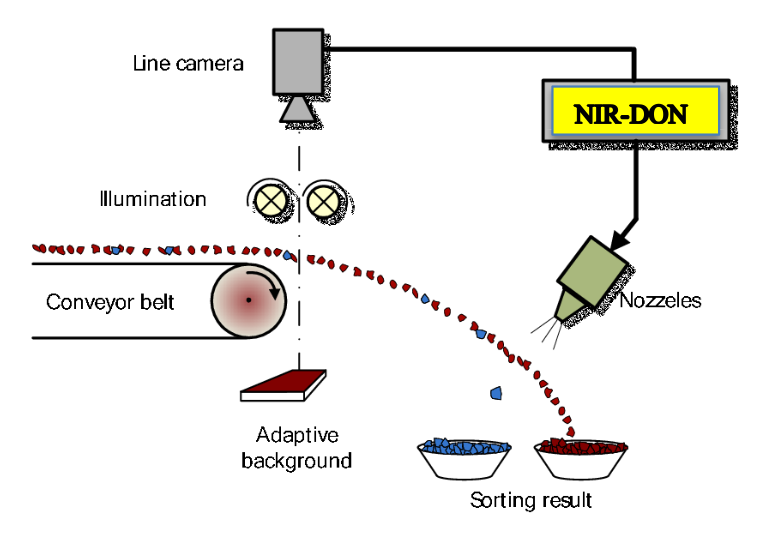
\includegraphics[width=0.7\linewidth]{media/images/esquema-del-sistema.png}
    \caption{Esquema del sistema de detección y filtrado de granos contaminados}\ \label{fig:detection-system}
\end{figure}


\subsection{NIR-HSI}


\gls{nir-hsi} es una tecnología rápida, no destructiva y precisa que nos permite hacer inspecciones de calidad, la cual ha demostrado su potencial en los últimos años\ \cite{Applicat5:online}. 
Es una técnica de imagen química basada en la espectroscopia de reflectancia (la luz reflejada por los materiales), la cual es capaz de caracterizar compuestos orgánicos y algunos minerales\ \cite{NIRHyper23:online}. Este método puede resultar mucho más directo, pues es rápido y no requiere análisis químico; barato, por los mismos motivos; y preciso, pues permite analizar los granos individualmente y no en lote; que el análisis químico.

Como hemos comentado en la introducción, nuestro objetivo es conseguir un modelo que, utilizando \gls{nir-hsi}, prediga lo mejor posible qué granos de una \gls{imagen hiperespectral} contienen granos contaminados con \acrshort{don}. Para ello, partimos con una base de datos de imágenes hiperespectrales con formato \acrshort{bil}, las cuales simulan las imágenes tomadas en la cadena de producción y de las cuáles podemos extraer la información de los píxeles que forman los granos.
Los archivos con formato \acrshort{bil} albergan los datos hiperespectrales de una imagen, como podemos ver en la \textit{figura \ref{fig:bil-example}}. Es decir, para las diferentes bandas especificadas, contiene la información de cada píxel que forma la imagen. Para ello, hace uso de otro archivo complementario con formato \textit{bil.hdr} que brinda información sobre este, como las diferentes bandas (frecuencias, en nuestro caso son 168) presentes en la imagen, entre otros. Una vez sabemos qué formato tienen los datos, podemos leer los archivos \acrshort{bil} que tenemos y formar un \acrshort{csv} con los datos centralizados para que nos sea más fácil trabajar con ellos. Para no tener un archivo demasiado grande, hemos desechado los píxeles que forman parte del `fondo' negro de la imagen, para determinar si un píxel es fondo, se hace la media de todos los valores de las reflectancias para ese píxel y si no pasa un umbral trivial, lo consideramos parte del fondo.

Una vez tenemos el \acrshort{dataset} con los datos de cada píxel, podemos generar un nuevo \acrshort{dataset} que agrupe los píxeles en grupos, o granos. De esta forma, podemos añadir un nuevo filtro que consista en que los granos deben de tener un tamaño mínimo (en píxeles), es decir, podemos desechar los granos que sean demasiado pequeños ya que probablemente sea ruido en la imagen. De esta forma, agruparíamos \textit{N} filas de datos de píxeles, en tan solo una fila conservando la media de cada columna.

\begin{figure}[!ht]
    \centering
    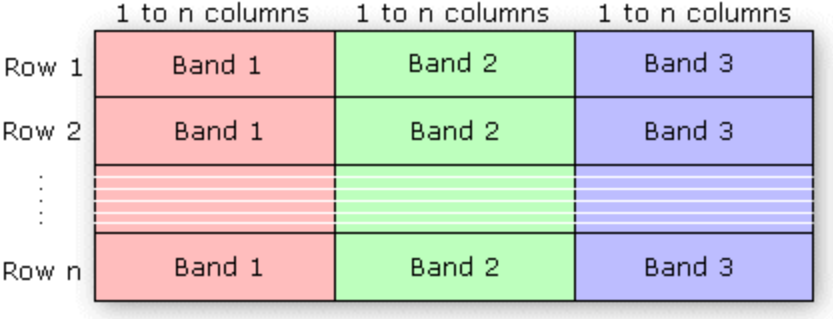
\includegraphics[width=0.7\linewidth]{media/images/bil.png}
    \caption{Formato de los datos en un archivo \acrshort{bil}. Fuente \cite{Archivos82:online}}\ \label{fig:bil-example}
\end{figure}

Por otro lado, tenemos una base de datos con el estado de contaminación de estos mismos granos. A partir de ahora utilizaremos los términos contaminación y etiqueta como sinónimos a la hora de referirnos a los granos.


\subsection{Contaminación del grano}\ \label{sec:separacion}

El valor de contaminación \acrshort{don} de una muestra se obtiene, como hemos comentado anteriormente, realizando un análisis químico por lotes. Este análisis nos devuelve el valor de la concentración de \acrshort{don} en el lote, de modo que si supera los \(1250\ \mu g/kg\), por ley, la muestra se considera contaminada. Sabiendo esto, previamente en laboratorio se ha realizado un análisis de los granos que forman las imágenes \acrshort{bil} que tenemos y, por lo tanto, además de los datos hiperespectrales, sabemos el nivel de contaminación que posee cada grano y lo podemos agregar como columna en el \acrshort{csv} que tenemos.


Al ser el valor de contaminación el que queremos predecir, a partir de ahora utilizaremos los términos contaminación y etiqueta como sinónimos. Además agregaremos otra columna, también de contaminación, la cual será \textit{booleana}, en lugar de un valor contínuo, y nos indicará si el valor concentración de ese grano supera el umbral legal comentado anteriormente. De esta forma, podemos plantear el problema tanto por regresión como por clasificación, 


\subsection{Análisis del mercado potencial}






\section{Marco teórico, conceptos clave del ML}

\begin{quote}
    `\gls{ml}: the use and development of computer systems that are able to learn and adapt without following explicit instructions, by using algorithms and statistical models to analyse and draw inferences from patterns in data'\ \cite{machinel18:online}
\end{quote}

Es decir, un sistema que es capaz de inferir patrones de unos datos y realizar predicciones sobre nuevos datos a raíz de los patrones encontrados. 


\subsection{Tipos de aprendizaje y modelos}

Hay cuatro tipos de aprendizaje en el ML:\@ supervisado, no supervisado, semi-supervisado y de refuerzo\ \cite{homl56}.

Como parte de nuestros datos están etiquetados, podemos utilizar tanto el aprendizaje supervisado como el semi-supervisado. En un sistema supervisado se requiere que todos los datos estén etiquetados con la categoría deseada, en nuestro caso la contaminación. Sin embargo, para el semi-supervisado no es necesario que todos los datos estén etiquetados, pues utilizan tanto los datos etiquetados como los que no (datos parcialmente etiquetados) para tratar de generalizar mejor\ \cite{homl56}.

No utilizaremos el no supervisado, pues consiste en un conjunto de técnicas utilizadas para agrupar automáticamente datos no etiquetados a base de similitudes sin tener supervisión previa. El objetivo es que los datos dentro de un mismo grupo sean más similares entre sí que con los otros grupos\ \cite{Clustera13:online}. Sin embargo, como tenemos una cantidad más o menos considerable de información etiquetada, no nos hace falta.

Tampoco utilizaremos el aprendizaje por refuerzo, pues no se encuentra implementado dentro de la librería que utilizamos \textit{\href{https://scikit-learn.org/stable/}{sklearn}} y tampoco está dentro de los objetivos del proyecto.


\subsection{Fases del desarrollo de un proyecto de ML}

Nuestro proyecto ha tenido las fases que nombramos a continuación:

\begin{enumerate}
    \item Obtención de datos (\textit{apartado\ \ref{sec:obtencion}})
        \begin{enumerate}
            \item Recolección de información de los \acrshort{bil}.
        \end{enumerate}
    \item Preparación de datos (\textit{apartado\ \ref{sec:preprocesado}})
        \begin{enumerate}
            \item Selección de métodos de preprocesado
        \end{enumerate}
    \item Entrenamiento de los modelos (\textit{apartado\ \ref{sec:entrenamiento}})
        \begin{enumerate}
            \item Entrenamiento `básico' de modelos
            \item Selección y refinamiento
        \end{enumerate}
    \item Evaluación de resultados
        
    \item Monitoreo de los modelos
\end{enumerate}

Podemos generalizar los procesos de un proyecto de \gls{ml} meidnate el esquema de la \textit{Figura\ \ref{fig:ml-development-cycle}}. Cabe destacar que el proceso de entrenar un modelo de \gls{ml}, como bien muestra la imagen, es un proceso cíclico en búsqueda de mejores resultados a base de probar metodologías distintas, añadir pasos, el cambio de requisitos, etc.

\begin{figure}[!htb]
    \centering
    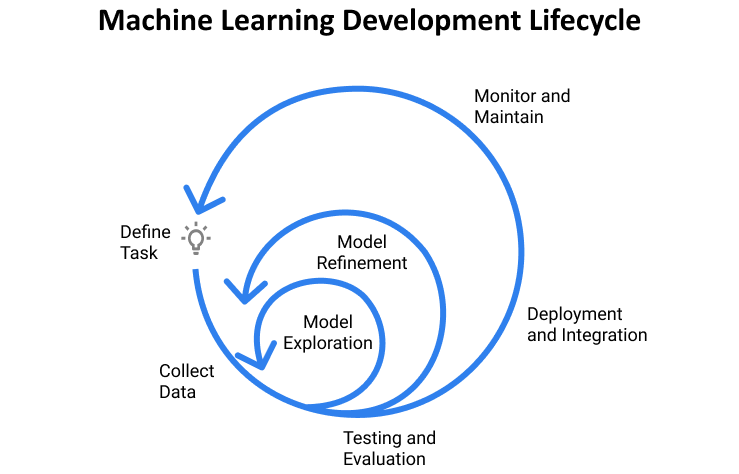
\includegraphics[width=\linewidth]{media/images/ml-development-cycle.png}
    \caption{Esquema del proceso del desarrollo de un proyecto de \gls{ml}, fuente\ \cite{Organizi22:online}}\ \label{fig:ml-development-cycle}
\end{figure}


\subsection{Métricas de evaluación de modelos}

Antes de continuar con el entrenamiento de modelos, su mejora y la selección de pasos del preprocesado; necesitamos algún tipo de métrica para evaluar y comparar los resultados. A continuación, explicaremos las que hemos utilizado para los diferentes tipos de modelos.

\subsubsection{Clasificación supervisada y semi-supervisada}\ \label{sec:classification-metrics}

Primeramente, explicaremos las partes de una matriz de confusión como la que podemos ver en la \textit{Figura\ \ref{fig:confusion-matrix-example}}. Podemos ver que tiene cuatro partes:

\begin{itemize}
    \item \textit{True Positive (tp)}, las muestras que el modelo clasifica como positivas que realmente son positivas.
    \item \textit{False Positive (fp)}, las muestras que el modelo clasifica como positivas que realmente son negativas.
    \item \textit{True Negative (tn)}, las muestras que el modelo clasifica como negativas que realmente son negativas.
    \item \textit{False Negative (fn)}, las muestras que el modelo clasifica como negativas que realmente son positivas.
\end{itemize}

Estos cuatro valores son la base del resto de métricas que comentaremos a continuación.

\begin{figure}[!ht]
    \centering
    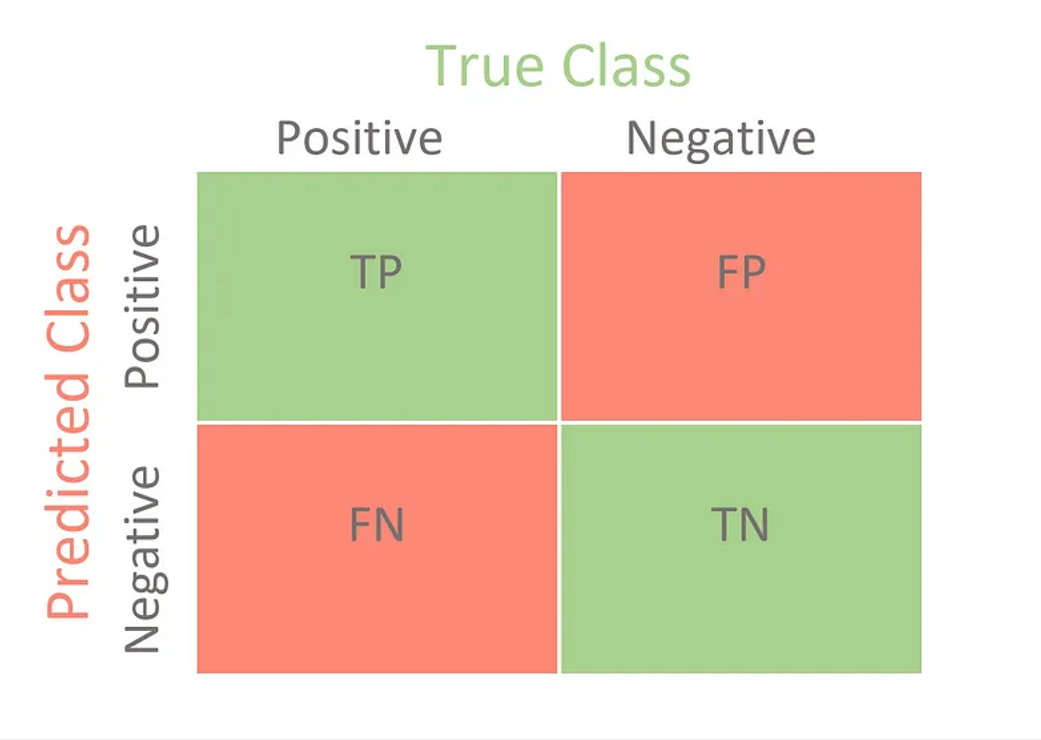
\includegraphics[width=0.7\linewidth]{media/images/confusion-matrix-example.png}
    \caption{Ejemplo de matriz de confusión, fuente\ \cite{Confusio71:online}}\ \label{fig:confusion-matrix-example}
\end{figure}

Antes de continuar con las métricas que compararemos, comentaremos también otras más básicas que son utilizadas para calcular las que utilizaremos\ \cite{Precisio23:online}.
\\ \textit{\textbf{Sensitivity}} permite saber la probabilidad de que una predicción positiva sea realmente positiva.
    \begin{equation}
        sensitivity=tp/(tp+fn)
    \end{equation}
\textit{\textbf{Specificity}} permite saber la probabilidad de que una predicción negativa sea realmente negativa.
\begin{equation}
        specificity=tn/(tn+fp)
    \end{equation}
\textit{\textbf{Recall}} indica la capacidad del modelo para encontrar todas las muestras positivas. 
    \begin{equation}
        recall=tp/(tp+fn)
    \end{equation}
\textit{\textbf{Precision}} indica la precisión de las predicciones positivas, es decir, la habilidad del clasificador para no predecir como positiva una muestra que es negativa.
    \begin{equation}
        precision=tp/(tp+fp)
    \end{equation}

Con estas métricas básicas podemos definir las que realmente compararemos, ya que tienen en cuenta el balanceo del \gls{dataset}:

\textit{\textbf{fbeta score}} es la media harmónica ponderada entre \textit{\textbf{Precision}} y \textit{Recall}. 
El parámetro \textit{beta} representa la importancia de \textit{Recall} por encima de \textit{Precision}. 
Es decir, \(beta>1\) le da más importancia a \textit{Recall} y, contrariamente, \(beta<1\) le da más peso a \textit{Precision}.\ \cite{FscoreWi30:online}
    \begin{equation}
        f_\beta = (1 + \beta^2)*\frac{precision*recall}{(\beta^2*precision)+recall}
    \end{equation}

Para comparar los modelos utilizaremos el parámetro \textit{beta} con valor de \textit{2}, pues consideramos más importante el \textit{Recall}, ya que creemos que los falsos negativos son peores que los falsos positivos. Es decir, consideramos peor que el modelo no detecte una muestra contaminada que detecte una muestra como contaminada cuando no lo es.

\textit{\textbf{Balanced accuracy}} es la media aritmética de \textit{Sensitivity} y \textit{Specificity}. Se utiliza principalmente cuando tratamos con datos desbalanceados.\ \cite{Balanced44:online} Su valor representa la exactitud media del modelo en las diferentes clases representadas por los datos, en nuestro caso, la clase de ``CONTAMINADO'' o ``NO CONTAMINADO''. Este valor, representa la exactitud con la que el modelo es capaz de clasificar las muestras de las diferentes clases, teniendo en cuenta la distribución de la clase mayoritaria. Es decir, si el valor de \textit{balanced accuracy} se acerca al 1, el modelo es capaz de clasificar correctamente las muestras de las diferentes clases, mientras que si se acerca a 0, el modelo no es capaz de clasificar correctamente las muestras o se aprovecha del desbalance de los datos, prediciendo mucho más la clase mayoritaria.
\begin{equation}
    balanced\_accuracy =\frac{sensitivity + specificity}{2}
\end{equation}

\section{Diseño del proyecto}

\subsection{Análisis del problema y de los datos}\label{sec:obtencion}

Considerando que los datos contenidos en los archivos con formato \gls{bil} contienen 168 columnas con información de las diferentes longitudes de onda\ \cite{WhatIsHy18:online} y además el nivel de contaminación \gls{don} de cada grano, podemos generar un \gls{dataset} con los datos de cada grano, haciendo la media de cada longitud de onda por cada píxel del mismo grano. Una vez hemos extraído la información de todos los archivos \gls{bil} y la hemos guardado en un archivo \acrshort{csv}, podemos entrenar los modelos sobre este.

Cabe recalcar que el nivel de contaminación \gls{don} es un valor entero, por lo tanto, para entrenar tanto los modelos de clasificación como los de regresión, lo hemos guardado en dos columnas, una con el valor exacto y otra con un valor binario que indica si el grano está contaminado o no.

\subsection{Preprocesado de datos}\label{sec:preprocesado}

Ahora que tenemos los datos en un solo archivo \acrshort{csv}, el siguiente paso es preprocesarlos. Para ello, hemos realizado los siguientes pasos: 

\begin{enumerate}
    \item Eliminación de columnas
    \item Codificación
    \item Valores atípicos (\textit{outliers})
    \item Separación en datos de entreno y de prueba (\textit{train-test-split})
    \item Balanceo de datos
    \item Preprocesado común, (\textit{pipeline})
    \begin{enumerate}
        \item Separación de datos aplicando la primera derivada 
        \item Aumento de dimensionalidad (\textit{Polynomial Features})
        \item Estandarización  (\textit{Standard Scaler})
        \item Reducción de dimensionalidad (\textit{Principal Component Analysis})
    \end{enumerate}
    
\end{enumerate}


\subsubsection{Eliminación de columnas, codificación y valores atípicos}

Existen datos que nos interesan como medida de seguridad, pero no nos interesa que un modelo entrene con ellos, ya que podría inferir patrones irreales o incluso memorizarlos. En nuestro caso, un ejemplo sería una columna que indicase el número identificador del grano o el archivo del cual se han extraído los datos.

La codificación consiste en transformar columnas con datos categóricos en columnas de datos numéricos, pues los modelos de \acrshort{ml} funcionan mejor con valores numéricos. En nuestro caso, la única columna con valores no numéricos era la columna de la contaminación, que podía tomar los valores \textit{\{B, C\}}, así que lo codificamos manualmente como se muestra a continuación:

{
    \centering
    \textit{B \longrightarrow{} 0}, \textit{C \longrightarrow{} 1}\par
}

Los valores atípicos u \textit{outliers} son aquellos valores inusuales en los datos que pueden distorsionar nuestros análisis estadísticos. Sin embargo, se debe tener en cuenta que puede haber mucha variación en la naturaleza de nuestro problema. Por ello, se deben diferenciar los \textit{outliers} que se pueden incluir en los datos y los que no. En nuestro caso, no hemos quitado ningún \textit{outlier}, pues la mayoría de granos tenía alguna columna de datos que no entraba dentro de lo ``normal'', como por ejemplo se puede observar en la \textit{Figura\ \ref{fig:outliers}}. Por lo que después de probar a quitar todos los granos que alguna de sus columnas fuera un \textit{outlier} (con el \textit{Código\ \ref{code:zscore}}), nos quedamos sin datos.

\begin{figure}[!h]
    \centering
    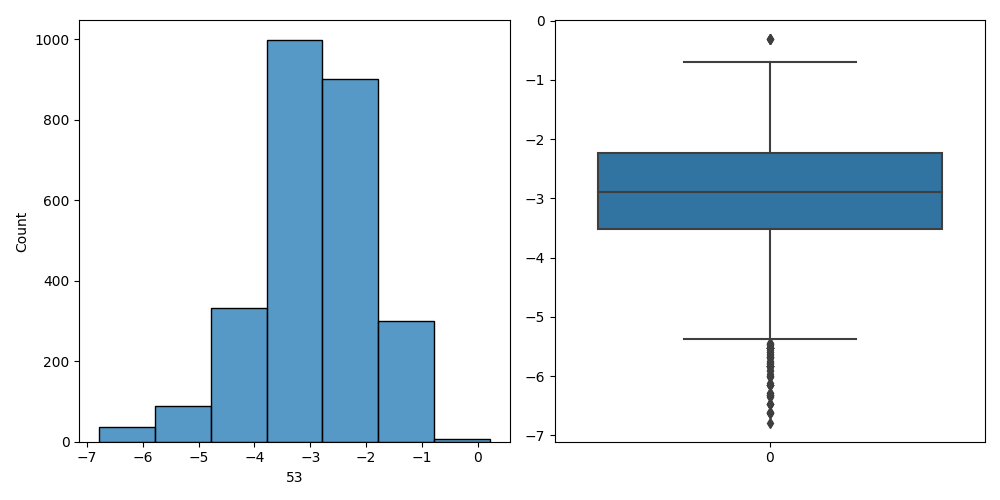
\includegraphics[width=0.7\linewidth]{media/images/col-53-outliers.png}
    \caption{Representación de los \textit{outliers} de la columna 53 en un gráfico de velas, fuente propia, \textit{Código\ \ref{code:plot-outliers}}}\ \label{fig:outliers}
\end{figure}


\subsubsection{Separación de datos de entreno y de prueba}

En todo el proyecto hemos estado utilizando la librería \href{https://scikit-learn.org/stable/}{sklearn}, esta tiene un submódulo con una función \href{https://scikit-learn.org/stable/modules/generated/sklearn.model_selection.train_test_split.html}{sklearn.model\_selection.train\_test\_split} para separar el \gls{dataset} en entreno y prueba. De esta función, lo más importante es que nos permite la opción de utilizar \textit{stratify}, la cual es muy recomendable cuando el \textit{dataset} no está balanceado.

De todas las opciones, cabe recalcar una que hemos habilitado, pues como en el \gls{dataset} original las etiquetas no están balanceadas y hay muchos más granos sanos que contaminados, es importante que los granos contaminados estén igualmente representados tanto en el conjunto de prueba como en el de entreno, esto se consigue con la opción \textit{stratify}.


\subsubsection{Balanceo de datos}

Podemos ver en la \textit{Figura\ \ref{fig:unbalance}} que los datos no están balanceados, es decir, que la columna que nos interesa `Contaminación' no tiene un número de datos similares en cada clase. En nuestro caso, como en general es más complicado encontrarse un grano contaminado, tenemos más granos sanos.

\begin{figure}[!h]
    \centering
    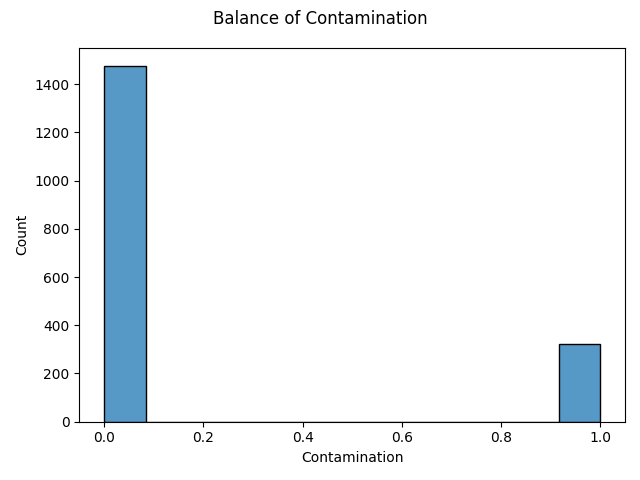
\includegraphics[width=0.5\linewidth]{media/images/unabalance.png}
    \caption{Balanceo de la clase objetivo del \gls{dataset}, fuente propia}\ \label{fig:unbalance}
\end{figure}

Al tener las clases desbalanceadas tenemos varias opciones:
\begin{enumerate}
    \item Usar métodos de evaluación que tengan en cuenta el desbalance de las clases.
    \item Balancear el \gls{dataset} utilizando tanto \textit{undersampling} como \textit{oversampling}.
\end{enumerate}

La toma de nuevos datos es costosa y como tenemos relativamente pocos para la cantidad de columnas (las 168 longitudes de onda), el balanceo de datos es esencial. Sorteamos este problema utilizando métricas que tienen en cuenta el balance de los datos. Sin embargo, podemos balancear los datos en dos pasos: \textit{undersampling} y \textit{oversampling}. 

Como su nombre indica, \textit{undersampling} es una técnica para reducir las muestras de la clase mayoritaria, en nuestro caso los granos sin contaminar. Existen varias técnicas para hacer \textit{undersampling}, las cuales comentaremos en la \textit{sección\ \ref{sec:undersampling}}. Por otro lado, el \textit{oversampling} consiste en la creación de datos sintéticos, similares a los reales, para suplir la diferencia de balanceo entre las diferentes clases. Al igual que con el \textit{undersampling}, existen diversas técnicas que comentaremos más adelante en la \textit{sección\ \ref{sec:oversampling}}.

\paragraph{Undersampling}\ \label{sec:undersampling}


A la hora de balancear los datos, buscamos, de alguna forma, reducir la diferencia en el número de muestras en las diferentes clases del dataset. En el paso de \textit{undersampling}, buscamos reducir la cantidad de muestras de las clases mayoritarias. Para ello, debemos de alguna forma determinar qué muestras de las clases mayoritarias son más redundantes para evitar eliminar muestras `críticas'. Para ello hemos decidido utilizar los algoritmos de la librería \href{https://imbalanced-learn.org/stable/}{imblearn} que fue diseñada específicamente para los problemas de clasificación sobre \textit{datasets} desbalanceados.\ \cite{3Undersa98:online}

El primer algoritmo que probaremos será \textit{RandomUnderSampler}, el cual consiste en seleccionar un subconjunto aleatorio de datos. Para intentar no eliminar datos importantes como hemos comentado antes, hay otra versión que aplica una de las tres versiones de la heurística \textit{NearMiss}\ \cite{3Undersa98:online}, la cual se basa en el algoritmo \textit{nearest neighbors}:

\begin{enumerate}
    \item La versión \textbf{NearMiss1} elimina aquellos datos cuya distancia media a sus \textit{N} vecinos más cercanos de la clase minoritaria sea menor.
    \item La versión \textbf{NearMiss2} es parecida a la \textbf{1}, pero en esta la distancia media se computa sobre los \textit{N} vecinos más lejanos de la clase minoritaria.
    \item La versión \textbf{NearMiss3} consta de dos pasos, primero, de cada elemento de la clase minoritaria selecciona los \textit{M} vecinos más cercanos de la clase mayoritaria. Luego, por cada muestra seleccionada se calcula la distancia media respecto a los \textit{N} vecinos más cercanos de la clase minoritaria y se eliminan los que, de media, estén más alejados.
\end{enumerate}

El siguiente algoritmo, \textit{Tomek Links}, detecta los llamados \textit{Tomek Links}, estos son enlaces entre dos muestras de diferente clase, pongamos \(x\) e \(y\), definidos tal que para cualquier muestra \(z\): 
\[d(x,y) < d(x,z)\ and\ d(x,y) < d(y,z)\], donde \(d(a, b)\) es la distancia entre la muestra \(a\) y \(b\). En resumen, un \textit{Tomek Link} se da entre las muestras de distintas clases más cercanas entre sí. Este algoritmo suele ser bueno a la hora de eliminar ruido en los datos.

Por último, el algoritmo \textit{Edited Nearest Neighbours} elimina las muestras que no se parezcan demasiado a sus vecinos\ \cite{Wil72}. Para ello, comprueba para cada muestra que sus \textit{N} vecinos más cercanos sean de su misma clase, si no se cumple,podemos elegir si nos quedamos con las muestras de la clase mayoritaria o si eliminamos todas las muestras.


\paragraph{Oversampling}\ \label{sec:oversampling}

El segundo paso es el \textit{oversampling}, el cual consiste en la creación de los datos sintéticos para suplir la carencia de datos de las clases minoritarias. Al igual que en el paso anterior, hay algoritmos para realizar estas técnicas implementados en la librería \textit{imblearn}, sin embargo preferimos utilizar \href{https://sdv.dev/}{The Synthetic Data Vault} \cite{Synthesi69:online}, pues tiene mejor documentación y tiene un método sencillo para evaluar los datos generados. 

En la librería hay cuatro sintetizadores de datos que probaremos y son los siguientes:

\begin{enumerate}
    \item \textit{Gaussian Copula Synthesizer} \cite{Gaussian4:online}, el cual utiliza métodos estadísticos clásicos.
    \item \textit{TVAESynthesizer} \cite{TVAESynt0:online}, basado en \textit{VAE} \cite{Variatio61:online}, utiliza técnicas de redes neuronales.
    \item \textit{CTGANSynthesizer} \cite{CTGANSyn50:online} y \textit{CopulaGAN} \cite{CopulaGA37:online}, ambos utilizan métodos de \textit{deep learning} basados en \textit{GAN} \cite{Generati72:online}, los comentamos por encima pues no los probaremos porque no son recomendables para datasets con tantas columnas no discretas, pues generarían un dataset con muchísimas más columnas (en nuestro caso, multiplicarían las columnas por once, es decir, tendríamos 1848). 
\end{enumerate}

Una vez aumentado el dataset con los datos sintéticos, evaluaremos cuál es mejor para nuestro problema comparando la similitud de los datos generados con los reales y la calidad de los modelos resultantes de entrenar con el nuevo dataset.


\subsubsection{Preprocesado común}

Después de balancear los datos, debemos modificarlos para que tengan algunas propiedades que suelen ser preferibles a la hora de entrenar ciertos modelos. Es decir, hay modelos que les vendrá mejor tener los datos estandarizados, por ejemplo, y otros que no hará falta o será contraproducente, al final será la experiencia lo que nos diga qué pasos son preferibles.

Antes de comentar las diferentes formas de preprocesado de los datos, hemos preparado un entorno para entrenar una batería de modelos distintos sobre estos para ver y comparar su efectividad. Esta comparación de los modelos resultantes la haremos con las métricas que hemos comentado anteriormente.


Los pasos que hemos probado para preprocesar los datos son los que comentamos en las siguientes secciones.

\paragraph{Primera derivada}

Un primer paso recomendado desde el laboratorio, ya que era lo que utilizaban ellos en su modelo estadístico, es aplicar la primera derivada. El hacerlo permite mínimamente separar los granos contaminados de los que no, pues aplicar la derivada suaviza los datos, eliminando parte del ruido y dejando solo las tendencias.

% //TODO: Añadir ejemplo gráfico de la derivada

\paragraph{Transformada}

El siguiente paso que podemos probar es aplicar la transformada, como los resultados habiendo derivado los datos son mejores, transformaremos los datos después de derivarlos. La transformada consiste en transformar cada columna para que tengan una forma gaussiana\ \cite{sklearnp39:online}, a continuación mostraremos por qué, a grandes rasgos, esta forma es interesante. \cite{TheRoleo87:online}

\begin{enumerate}
    \item \textit{Realismo}, en muchos problemas con datos reales, la distribución de los datos es gaussiana.
    \item \textit{Propiedades estadísticas}, la forma de campana (o gaussiana) tiene propiedades conocidas que permiten la aplicación de varias técnicas estadísticas.
    \item \textit{Compatibilidad}, muchos modelos estadísticos y de \gls{ml} asumen que los datos tienen una distribución gaussiana.
\end{enumerate}

Como estamos utilizando \textit{sklearn}, tenemos una clase que nos aplica la transformada \href{https://scikit-learn.org/stable/modules/generated/sklearn.preprocessing.PowerTransformer.html}{sklearn.preprocessing.PowerTransformer}, por defecto esta clase además te aplica una estandardización de los datos, pero la hemos deshabilitado para aplicarla en el siguiente paso. 


\paragraph{Estandarización}

A continuación, probaremos la estandarización de los datos como hemos comentado anteriormente. Utilizaremos la clase \href{https://scikit-learn.org/stable/modules/generated/sklearn.preprocessing.StandardScaler.html}{sklearn.preprocessing.StandardScaler}. La estandardización consiste en el centrado y escalado de los datos. Para ello, columna por columna, restamos la media de los valores (centramos en torno al 0) y los dividimos por la varianza (para que la desviación tienda a 1). Tener los datos estandarizados suele ser un requisito para obtener buenos resultados al entrenar algunos modelos.\ \cite{sklearnp24:online}


\paragraph{Disminución y aumento de dimensionalidad}

Por último, podemos probar dos pasos que suelen ir juntos. El primero, \href{https://scikit-learn.org/stable/modules/generated/sklearn.preprocessing.PolynomialFeatures.html}{sklearn.preprocessing.PolynomialFeatures}, nos permite generar nuevas columnas de datos que consisten en combinar las demás columnas, multiplicándolas entre sí y elevando a un grado específico (segundo grado en nuestro caso). De esta forma, de nuestro \gls{dataset} de 168 columnas, obtenemos uno de 14365 columnas. Por ello, debemos aplicar el segundo y último paso para reducir la dimensionalidad de los datos y poder entrenar modelos en un tiempo razonable. Este paso es \href{https://scikit-learn.org/stable/modules/generated/sklearn.decomposition.PCA.html}{sklearn.decomposition.PCA} o \textit{Principal Component Analysis}, el cual reduce la dimensionalidad proyectando los datos a una espacio de menor dimensionalidad. Podemos leer algo más al respecto sobre \textit{PCA} en \ \cite{Principa62:online}. 
\section{Experimentación}

En esta sección mostraremos los resultados de las pruebas con los distintos métodos de preprocesado de datos y modelos; con el objetivo de encontrar la combinación que nos dé los mejores resultados.

Antes de comentar específicamente los distintos métodos que probaremos, explicaremos la forma en la que se han realizado estas pruebas.

Como hemos comentado anteriormente, separamos los datos de entreno y prueba aplicando la opción de \textit{stratify} y con una proporción de \textit{75/25\%} respectivamente.

Una vez separados los conjuntos de datos, los tenemos que preprocesar. Para ello, hemos utilizado el objeto \textit{Pipeline} \cite{sklearnp32:online}, el cual nos permite encadenar diferentes pasos de preprocesado para entrenar diferentes modelos de forma sencilla. Por ejemplo, si queremos probar diferentes modelos, podemos hacerlo de la siguiente forma: 

\begin{enumerate}
    \item Instanciamos los objetos de las diferentes clases de preprocesado que queramos probar con sus respectivos valores. En el caso excepcional de la \textit{primera derivada}, hemos creado nuestro propio \textit{Transformer} (objeto de ``preprocesado'') que aplica la derivada a los datos.
    \item Los agregamos a la \textit{Pipeline} en orden.
    \item Ajustamos la \textit{Pipeline} sobre el conjunto de datos de entreno.
    \item Aplicamos la \textit{Pipeline} ya configurada sobre los datos de entreno y prueba. 
\end{enumerate}


El \textit{Pipeline} nos ofrece la ventaja de poder guardar y cargar tanto el orden del procedimiento, como la configuración de los pasos intermedios para aplicarlos más adelante de forma sencilla. Por ejemplo el \textit{StandardScaler}, para modificar los datos de forma que tengan media 0 y varianza 1, guarda la media y la varianza de cada columna para poder aplicarla más adelante.

Vale la pena comentar también que este objeto de \textit{Pipeline} nos ayuda a compartir la configuración del preprocesado entre la aplicación de entrenamiento de modelos y la de visualización de las predicciones sobre los archivos \gls{bil}.

Una vez hemos preprocesado los datos y entrenado los modelos; para evaluarlos, hemos utilizado la métrica \textit{Balanced Accuracy}, la cual hemos comentado en la \textit{Sección\ \ref{sec:classification-metrics}}.


\subsection{Análisis del impacto de la primera derivada}

Para probar que, como hemos comentado antes, el aplicar la primera derivada sobre los datos nos puede ayudar a la hora de predecir, podemos comparar los resultados de entrenar con o sin derivar en la \textit{Tabla\ \ref{tab:nopreprocessing-derivative-results}}. En esta, podemos ver los resultados de entrenar la batería de modelos y su \textit{Balanced Accuracy} la cual ha mejorado un \textbf{2.255\%} respecto a no haber preprocesado los datos, por lo tanto, continuaremos aplicando la derivada en los siguientes pasos.

Además en la \textit{Tabla\ \ref{tab:nopreprocessing-derivative-results}} podemos ver un comportamiento que se repite, hay algunos modelos con un \textit{Balanced Accuracy} de $50$ (en nuestro caso es este valor, pues tenemos dos clases), lo cual nos indica que el modelo no ha sido capaz de predecir correctamente la clase minoritaria. Esto se debe a que los datos están desbalanceados y el modelo se aprovecha de ello, prediciendo siempre la clase mayoritaria.


\begin{table}[!ht]
    \centering
    \begin{tabular}{|c|c|c|}
        \hline
        & \textit{Derivative} & \textit{No preprocessing} \\ \hline
        Model Name & Balanced accuracy & Balanced accuracy \\ \hline
        XGBoost & 50 & 50 \\ 
        Stochastic Gradient Descent & 50 & 50 \\ 
        Random Forest & 66.531 & 70.069 \\ 
        Quadratic Discriminant Analysis & 50 & 50 \\ 
        Multi-Layer Perceptron & 51.114 & 50 \\ 
        Linear Discriminant Analysis & 53.96 & 54.306 \\ 
        LightGBM & 71.846 & 62.632 \\ 
        K-Neighbors & 71.289 & 82.46 \\ 
        Hist Gradient Boosting & 68.97 & 58.988 \\ 
        Extra Trees & 78.756 & 76.438 \\ 
        Decision Tree & \textbf{67.224} & 50 \\ \hline
        \textit{Average} & \textbf{61.790} & 59.535 \\ \hline
    \end{tabular}
    \caption{Comparación de los resultados de entrenar utilizando la derivada y sin preprocesar. Fuente propia.}\ \label{tab:nopreprocessing-derivative-results}
\end{table}

\subsection{Análisis del impacto de aplicar la transformada}

Podemos ver los resultados de entrenar utilizando la transformada sobre los datos derivados en la \textit{Tabla\ \ref{tab:derivative-transformed-results}}, vemos que la métrica \textit{Balanced Accuracy} en general empeora en un \textbf{1.12\%}, así que continuaremos las pruebas sin añadir la transformada al preprocesado.

\begin{table}[!h]
    \centering
    \begin{tabular}{|c|c|c|}
        \hline
            & \textit{Transformer \& derivative} & \textit{Derivative} \\ \hline
            Model Name & Balanced accuracy & Balanced accuracy \\ \hline
            XGBoost & 50 & 50 \\ 
            Stochastic Gradient Descent & 50 & 50 \\ 
            Random Forest & 66.531 & 66.531 \\ 
            Quadratic Discriminant Analysis & \textbf{55.149} & 50 \\ 
            Multi-Layer Perceptron & 50 & 51.114 \\ 
            Linear Discriminant Analysis & 52.529 & 53.96 \\ 
            LightGBM & 71.846 & 71.846 \\ 
            K-Neighbors & \textbf{56.143} & 71.289 \\ 
            Hist Gradient Boosting & 68.97 & 68.97 \\ 
            Extra Trees & 78.967 & 78.756 \\ 
            Decision Tree & 67.224 & 67.224 \\ \hline
            \textit{Average} & 60.669 & \textbf{61.790} \\ \hline
    \end{tabular}
    \caption{Comparación de los resultados de entrenar transformando y derivando los datos; frente a solo derivando. Fuente propia.}\ \label{tab:derivative-transformed-results}
\end{table}

\subsection{Análisis del impacto de la estandarización de los datos}

Al aplicar la estandarización de los datos después de derivarlos obtenemos los resultados de la \textit{Tabla\ \ref{tab:derivative-standarization-results}}, los cuales en general son notablementes mejores que los anteriores, viendo una mejora del \textbf{2.74\%} en la \textit{Balanced Accuracy}. Estas mejoras ocurren en los modelos marcados en la tabla, \textit{QDA} y \textit{MLP}.


\begin{table}[!h]
    \centering
    \begin{tabular}{|c|c|c|}
        \hline
        & \textit{Derivative \& Scaler} & \textit{Derivative} \\ \hline
        Model Name & Balanced accuracy & Balanced accuracy \\ \hline
        XGBoost & 50 & 50 \\
        Stochastic Gradient Descent & 49.834 & 50 \\ 
        Random Forest & 66.531 & 66.531 \\ 
        Quadratic Discriminant Analysis & \textbf{72.358} & 50 \\ 
        Multi-Layer Perceptron & \textbf{59.41} & 51.114 \\ 
        Linear Discriminant Analysis & 53.96 & 53.96 \\ 
        LightGBM & 71.981 & 71.846 \\ 
        K-Neighbors & 70.807 & 71.289 \\ 
        Hist Gradient Boosting & 68.97 & 68.97 \\ 
        Extra Trees & 78.756 & 78.756 \\ 
        Decision Tree & 67.224 & 67.224 \\ \hline
        \textit{Average} & \textbf{64.530} & 61.790 \\ \hline
    \end{tabular}
    \caption{Comparación de los resultados de entrenar derivando y estandarizando los datos; frente a solo derivando. Fuente propia.}\ \label{tab:derivative-standarization-results}
\end{table}


\subsection{Impacto del aumento y disminución de dimensionalidad de los datos}


Por último, aun siendo un paso generalmente recomendado, el aumento y disminución de dimensionalidad nos ha dado los resultados de la \textit{Tabla\ \ref{tab:derivative-standarization-dimensionality-results}}, los cuales son significativamente peores que los anteriores empeorando la \textit{Balanced Accuracy} en un \textbf{5.66\%}. Por lo tanto, continuaremos con los datos derivados y estandarizados sin aumentar o disminuir la dimensionalidad de los datos.

\begin{table}[!h]
    \centering
    \resizebox{\textwidth}{!}{\begin{tabular}{|c|c|c|}
        \hline
        & \textit{Derivative \& Scaler \& Polynomial Features \& PCA} & \textit{Derivative \& Scaler} \\ \hline
        Model Name & Balanced accuracy & Balanced accuracy \\ \hline
        XGBoost & 50 & 50 \\ 
        Stochastic Gradient Descent & 52.439 & 49.834 \\ 
        Random Forest & 61.939 & 66.531 \\ 
        Quadratic Discriminant Analysis & {63.234} & {72.358} \\ 
        Multi-Layer Perceptron & 54.682 & 59.41 \\ 
        Linear Discriminant Analysis & 50.903 & 53.96 \\ 
        LightGBM & {62.933} & {71.981} \\ 
        K-Neighbors & {64.092} & {70.807} \\ 
        Hist Gradient Boosting & 61.924 & 68.97 \\ 
        Extra Trees & 70.37 & 78.756 \\ 
        Decision Tree & 55.014 & 67.224 \\ \hline
        \textit{Average} & \textbf{58.866} & \textbf{64.530} \\ \hline
    \end{tabular}}
    \caption{Comparación de los resultados de entrenar derivando, estandarizando y ajustando la dimensionalidad de los datos; frente a solo derivando y estandarizando. Fuente propia.}\ \label{tab:derivative-standarization-dimensionality-results}
\end{table}


\subsection{Selección de modelos y \textit{hyperparameter tuning}}\ \label{sec:entrenamiento}

Una vez encontrada una combinación de pasos de preprocesado que nos mejora los resultados, podemos pasar al siguiente paso de selección de los modelos. Habiendo entrenado ya los modelos, vemos en la \textit{Tabla\ \ref{tab:final-training-results}} que algunos hacen \textit{overfitting}. El \textit{overfitting} ocurre cuando un modelo se ajusta demasiado a los datos con los que ha entrenado y no generaliza bien, es decir que predice mejor los datos con los que ha entrenado que datos nuevos. Esto lo podemos ver en la tabla comparando los valores de las columnas \textit{Train} y \textit{Test score}.

Donde lo podemos ver más claramente es en \textit{KNeighbors}, vemos en la \textit{Figura\ \ref{fig:lc-knn}} que, para cualquier cantidad de datos con los que entrenemos el modelo, siempre predecirá bien con los que ha entrenado y no tanto con los demás. Nuestro objetivo es intentar que ambos valores no sean tan dispares y que sean lo más altos posibles, para ello aplicaremos \textit{hyperparameter tuning}.

\begin{table}[!ht]
    \centering
    \begin{tabular}{|c|ccc|}
    \hline
        Model Name & Train score & Test score & Balanced accuracy \\ \hline
        XGBoost & 82 & 82 & 50 \\ 
        Stochastic Gradient Descent & 64.815 & 56.444 & 49.834 \\ 
        Random Forest & \textbf{99.926} & \textbf{87.778} & 66.531 \\ 
        Quadratic Discriminant Analysis & \textbf{96.148} & \textbf{83.111} & 72.358 \\ 
        Multi-Layer Perceptron & 90.815 & 84 & 59.41 \\ 
        Linear Discriminant Analysis & \textbf{85.333} & \textbf{78.222} & 53.96 \\ 
        LightGBM & 82.222 & 72.222 & 71.981 \\ 
        K-Neighbors & \textbf{100} & \textbf{86.889} & 70.807 \\ 
        Hist Gradient Boosting & \textbf{78.444} & \textbf{70.444} & 68.97 \\ 
        Extra Trees & \textbf{99.63} & \textbf{90.444} & 78.756 \\ 
        Decision Tree & 56.963 & 58.889 & 67.224 \\
    \hline
    \end{tabular}
    \caption{Tabla ampliada de los resultados de entrenar los modelos utilizando la derivada y \textit{StandardScaler}. Fuente propia.}\ \label{tab:final-training-results}
\end{table}

\begin{figure}[!h]
    \centering
    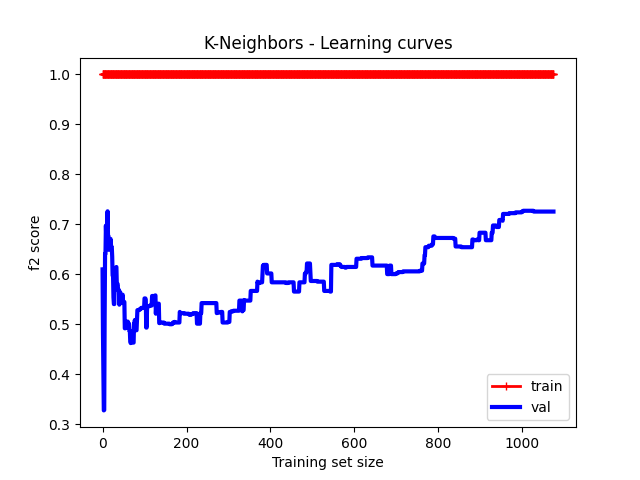
\includegraphics[width=0.7\linewidth]{media/images/learing-curves-knn.png}
    \caption{Gráfico de la curva de aprendizaje del modelo \textit{K-Neighbors} entrenándolo y probándolo sobre los datos de entreno únicamente. Fuente propia}\ \label{fig:lc-knn}
\end{figure}

El \textit{hyperparameter tuning} tiene como objetivo encontrar un conjunto de parámetros que maximice el rendimiento del modelo sobre los datos de prueba. En nuestro caso, como los datos están desbalanceados, podemos utilizar como función a optimizar el \textit{Balanced Accuracy}. Como cada modelo es distinto, debemos encontrar los parámetros adecuados para cada uno. 

Como no todos los modelos nos han dado buenos resultados y el \textit{hyperparameter tuning} es un proceso costoso, para ahorrarnos tiempo podemos utilizar solamente los mejores, como hemos visto en la \textit{Tabla\ \ref{tab:final-training-results}} hay modelos que tienen mejores resultados que otros. Así que escogeremos los cuatro con mejor \textit{balanced accuracy}, es decir: \textit{Extra Trees, Quadratic Discriminant Analysis, LightGBM y K-Neighbors}.

Realizaremos el \textit{hyperparameter tuning} en dos pasos, primeramente utilizaremos \textit{Random Search} y después \textit{Grid Search}, ya implementados en \textit{sklearn}.
Ambos métodos utilizan \textit{cross-validation}, una técnica para evitar el \textit{overfitting} (y el \textit{underfitting}) que consiste en la división de los datos de entreno en partes iguales.

Una vez divididos los datos de entreno en \textit{N} partes, se itera sobre cada una de ellas, utilizando \textit{N-1} partes para entrenar el modelo y la restante para evaluarlo. Una vez obtenemos los modelos entrenados sobre las diferentes partes, los comparamos con la función de rendimiento que queramos optimizar y seleccionamos el mejor. Una vez seleccionado el mejor modelo, lo probamos sobre los datos de prueba y obtenemos los resultados finales. Podemos ver este proceso gráficamente en la \textit{Figura\ \ref{fig:cross-validation}}.

\begin{figure}[!h]
    \centering
    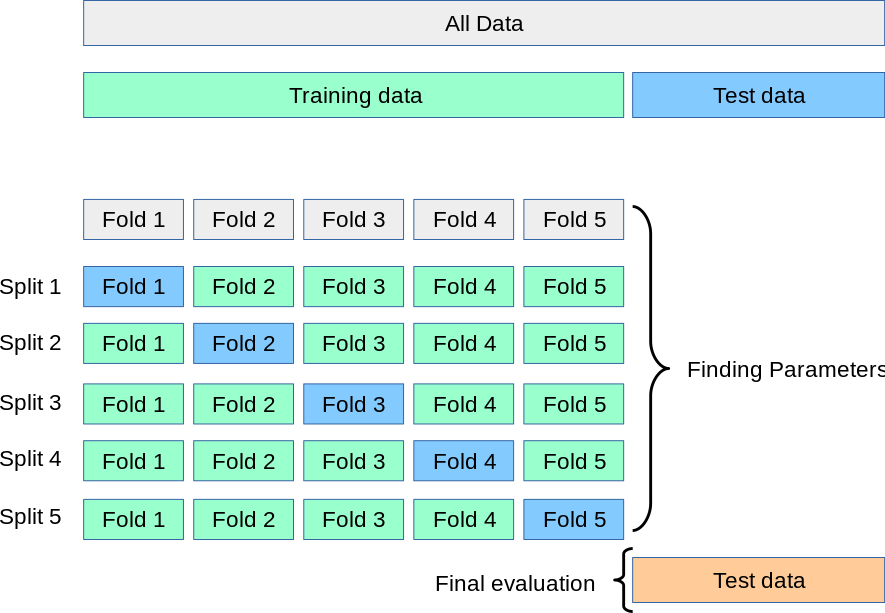
\includegraphics[width=0.7\linewidth]{media/images/cross-validation.png}
    \caption{\textit{Cross-validation} explicado gráficamente. Fuente:\ \cite{31Crossv20:online}}\ \label{fig:cross-validation}
\end{figure}


El \textit{random search} consiste en la búsqueda de estos parámetros habiendo definido un rango de posibilidades. Es decir, para cada parámetro que le queramos pasar al modelo definiremos un rango de valores que puede tener, entonces el \textit{random search} entrena el modelo repetidas veces con una permutación aleatoria de sus parámetros y se guarda los resultados. Podemos ver un ejemplo en el \textit{Código\ \ref{code:random-search-example}}.
Podemos ir probando diferentes parámetros y rangos hasta que estemos satisfechos con el resultado.


Una vez estemos contentos con los resultados, los refinaremos utilizando \textit{grid search}. A diferencia del \textit{random search}, el \textit{grid search} prueba todas las posibles combinaciones que le pasemos como parámetro y, consecuentemente, es mucho más lento. Por ello, utilizaremos el \textit{grid search} con los valores de los parámetros que dan los cinco mejores resultados del paso anterior, los cuales son potencialmente los mejores. Una vez definido un rango de parámetros para cada modelo seleccionado, obtenemos los resultados de la \textit{Tabla\ \ref{tab:hyperparameter-tuning-results}} donde vemos que los resultados del \textit{Random Search} y los de \textit{Grid Search} son iguales, salvo por \textit{Extra Trees}, en el cual el hacer \textit{Grid Search} sí que nos aporta mejores resultados. En general, vemos que hemos obtenido resultados parecidos a los de los modelos sin refinar, salvo por \textit{K-Neighbors}, que ha mejorado en un \textbf{19.467\%}, y \textit{Extra Trees}, que ha empeorado en un \textbf{12.586\%}.
Por lo tanto, deberíamos ajustar el rango de los parámetros que les pasamos a los modelos que no han dado buenos resultados y volver a entrenarlos hasta que estemos satisfechos. En nuestro caso no lo haremos, sino que retrocederemos unos pasos y probaremos otras técnicas.

\begin{table}[!h]
    \centering
    \resizebox{\textwidth}{!}{\begin{tabular}{|c|ccc|}
        \hline
        Model name & Train score & Test score & Balanced accuracy \\ \hline
        RS K-Neighbors & 100 & 90.274 & 90.274 \\ 
        GS K-Neighbors & 100 & 90.274 & 90.274 \\ 
        RS Quadratic Discriminant Analysis & 97.491 & 72.358 & 72.358 \\ 
        GS Quadratic Discriminant Analysis & 97.491 & 72.358 & 72.358 \\ 
        RS LightGBM & 86.013 & 71.018 & 71.018 \\ 
        GS LightGBM & 86.013 & 71.018 & 71.018 \\ 
        GS Extra Trees & 82.957 & 66.17 & 66.17 \\ 
        RS Extra Trees & 69.492 & 65.854 & 65.854 \\ \hline
        \end{tabular}}
    \caption{Resultados del primer entrenamiento con hyperparameter tuning. Fuente propia.}\ \label{tab:hyperparameter-tuning-results}
\end{table}
\clearpage

\subsection{Balanceo de datos}\ \label{sec:i2-balance}

\subsubsection{\textit{Undersampling}}

Al probar los algoritmos mencionados anteriormente, obtenemos los resultados de la \textit{Tabla\ \ref{tab:undersampling-methods}}. 
Hemos agregado una columna más, \textit{Avg. score diff}, que nos indica la diferencia entre el \textit{Train} y \textit{Test score} para decidir mejor, pues las \textit{Balanced Accuracy} nos daba resultados bastante parecidos. Esta ``nueva'' métrica no indica cuánto \textit{overfitting} hacen los modelos que se entrenan sobre el dataset generado, por lo tanto, cuanto más cercana a \textit{0} sea, mejor. Podemos ver que, en general, los diferentes \textit{Near Miss}, obtienen resultados bastante peores que los otros métodos. En cuanto a los otros tres algoritmos restantes, podemos ver que el \textit{Tomek Links} es el único que tiene mejores resultados que el \textit{dataset} sin hacer \textit{undersampling}, por lo tanto, continuaremos con este método.

\begin{table}[!ht]
    \centering
    \begin{tabular}{|c|cc|} \hline
        & Avg. score diff & Avg. Balanced Accuracy \\ \hline
        \textit{\textbf{No undersampling}} & 7.805 & 64.53 \\ 
        \textit{\textbf{TL}} & 7.950 & 65.236 \\ 
        \textit{ENN (MODE)} & 8.953 & 64.575 \\ 
        \textit{RUS} & 9.176 & 63.656 \\ 
        \textit{NM v3} & 9.883 & 61.999 \\ 
        \textit{ENN (ALL)} & 10.410 & 66.523 \\ 
        \textit{NM v1} & 35.263 & 62.754 \\ 
        \textit{NM v2} & 41.914 & 61.315 \\ \hline
    \end{tabular}
    \caption{Resultado de entrenar los modelos básicos sobre el \textit{dataset} reducido con los diferentes métodos. Fuente: propia.}\ \label{tab:undersampling-methods}
\end{table}

Una vez hemos aplicado \textit{Tomek Links} sobre el \textit{dataset}, nos quedamos con el número de muestras de la \textit{Figura\ \ref{fig:balance-tl}} y la \textit{Tabla\ \ref{tab:balance-tl-comparison}}; en las cuales podemos ver que tan solo se han eliminado $12$.

\begin{figure}[!ht]
    \centering
    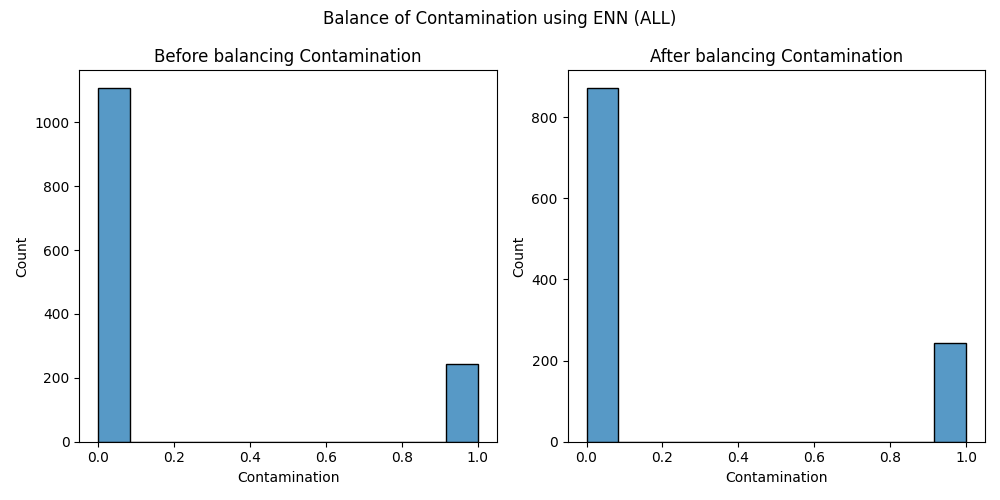
\includegraphics[width=0.8\linewidth]{media/images/balance.png}
    \caption{Comparación del balance de la clase objetivo antes y después de utilizar el método de \textit{undersampling ENN (ALL)}. Fuente propia.}\ \label{fig:balance-tl}
\end{figure}

\begin{table}
    \centering
    \begin{tabular}{|c|cc|} \hline
        & Good samples & Bad samples \\ \hline
        Before undersampling & 1107 & 243 \\
        After undersampling & 1095 & 243 \\ \hline
    \end{tabular}
    \caption{Comparación de las muestras antes y después de aplicar \textit{Tomek Links}. Fuente propia.}\ \label{tab:balance-tl-comparison}
\end{table}

\subsubsection{\textit{Oversampling}}

Para balancear el \textit{dataset}, como hemos comentado en la \textit{Sección\ \ref{sec:oversampling}}, hemos utilizado los sintetizadores de la librería \textit{sdv} para generar datos sintéticos. Además de los sintetizadores, la librería nos ofrece métodos para evaluar la calidad de los datos generados en forma de \textit{quality reports}. Estos \textit{quality reports} contienen la similitud estadística de los datos generados con los datos reales.

Una vez entrenados los sintetizadores y generados los datos, obtenemos los resultados de la \textit{Tabla\ \ref{tab:oversampling-quality-report}}, en los cuales podemos ver que la calidad de los datos generados por el sintetizador \textit{Gaussian Copula Synthesizer} son mejores.

\begin{table}[!ht]
    \centering
    \resizebox{0.8\linewidth}{!}{\begin{tabular}{|c|ccc|} \hline
        Synthesizer & Column Shapes & Column Pair Trends & Overall Quality \\ \hline
        Gaussian Copula Synthesizer & 94.75 & 99.83 & 97.29 \\
        TVAE Synthesizer & 84.37 & 74.97 & 79.64 \\ \hline
    \end{tabular}}
    \caption{Resultados del \textit{quality report} de los datos generados con los sintetizadores. Fuente propia}\ \label{tab:oversampling-quality-report}
\end{table}

Una vez tenemos los sintetizadores entrenados sobre la clase minoritaria, generamos nuevos datos y los añadimos al \textit{dataset} original, entrenamos los modelos básicos y obtenemos los resultados de la \textit{Tabla\ \ref{tab:balanced-basic-training}} donde podemos ver que, en general, los modelos resultantes son peores que los que se han entrenado con datos que no utilizan ningún sintetizador. Por lo tanto, mantendremos el \textit{undersampling}, pero no utilizaremos \textit{oversampling} en los siguientes pasos.

\begin{table}[!ht]
    \centering
    \begin{tabular}{|c|ccc|}\hline
        Model Name & Train score & Test score & Balanced accuracy \\ \hline
        XGBoost & 89.908 & 78.889 & 55.812 \\ 
        Stochastic Gradient Descent & 79.53 & 69.333 & 53.839 \\ 
        Random Forest & 97.42 & 82.444 & 66.17 \\ 
        Quadratic Discriminant Analysis & 93.005 & 82.667 & 53.779 \\ 
        Multi-Layer Perceptron & 94.209 & 80.889 & 64.74 \\ 
        Linear Discriminant Analysis & 87.041 & 76.889 & 53.628 \\ 
        LightGBM & 90.195 & 77.111 & 52.319 \\ 
        K-Neighbors & 100 & 85.778 & 76.393 \\ 
        Hist Gradient Boosting & 86.812 & 77.333 & 52.936 \\ 
        Extra Trees & 90.998 & 80 & 57.934 \\ 
        Decision Tree & 83.658 & 80.222 & 51.325 \\ \hline
        \textit{Average} & 90.252 & 79.232 & \textbf{58.079} \\ \hline
    \end{tabular}
    \caption{Resultados de entrenar los modelos básicos habiendo balanceado el \textit{dataset}. Fuente propia.}\ \label{tab:balanced-basic-training}
\end{table}

\subsection{Modelos \textit{ensemble}}

Hay dos tipos de modelos más complejos que no hemos probado que pueden darnos mejores resultados, estos son \textit{Voting Classifier} y \textit{Bagging Classifier}. El primero, \textit{Voting Classifier}, entrena los modelos que lo componen sobre el \textit{dataset} y, a la hora de predecir, extrapola su predicción en base a las predicciones de estos modelos. Es decir, realiza una votación y la clase que más se vote es la que sale como predicción como podemos ver en la \textit{Figura\ \ref{fig:voting-classifiers}}. Hay dos tipos de votación, \textit{hard} y \textit{soft}, \textit{hard} utiliza la clase predicha de los modelos, mientras que \textit{soft} suma las probabilidades de las clases a predecir y suele ser más preciso \cite{Ensemble96:online}. 

\begin{figure}[!h]
    \centering
    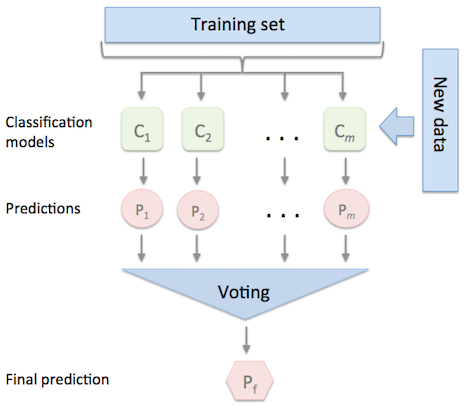
\includegraphics[width=0.7\linewidth]{media/images/majority_voting.png}
    \caption{Explicación gráfica del proceso de entreno y predicción de un \textit{Voting Classifier}. Fuente \cite{Ensemble96:online}.}\ \label{fig:voting-classifiers}
\end{figure}

Por otro lado el \textit{Bagging Classifier} entrena el mismo modelo sobre un subconjunto aleatorio del \textit{dataset} y luego agrega los resultados de las predicciones, ya sea haciendo la media o realizando una votación, para obtener una predicción final.\ \cite{sklearne53:online}


Antes de entrenar estos modelos, hemos de decidir qué otros modelos los compondran, por lo tanto, escogeremos los que han tenido mejores resultados al entrenarlos sobre el \textit{dataset} balanceado. Estos son los que mejores resultados tienen en la \textit{Tabla\ \ref{tab:tomeklinks-basic-training}}, es decir, \textit{K-Neighbors}, \textit{Quadratic Discriminant Analysis}, \textit{LightGBM} y \textit{Extra Trees}.

\begin{table}[!ht]
    \centering
    \begin{tabular}{|c|ccc|}
    \hline
        Model Name & Train score & Test score & Balanced accuracy \\ \hline
        XGBoost & 81.839 & 82 & 50 \\ 
        Stochastic Gradient Descent & 65.845 & 57.111 & 54.095 \\ 
        Random Forest & 100 & 86.444 & 63.791 \\ 
        \textbf{Quadratic Discriminant Analysis} & 96.487 & 83.778 & 72.282 \\ 
        Multi-Layer Perceptron & 90.284 & 82.889 & 60.659 \\ 
        Linear Discriminant Analysis & 85.202 & 77.778 & 54.17 \\ 
        \textbf{LightGBM} & 83.857 & 73.333 & 73.141 \\ 
        \textbf{K-Neighbors} & 100 & 87.111 & 71.424 \\ 
        Hist Gradient Boosting & 78.625 & 70.889 & 70.205 \\ 
        \textbf{Extra Trees} & 99.552 & 91.111 & 80.608 \\ 
        Decision Tree & 57.1 & 58.889 & 67.224 \\ \hline
    \end{tabular}
    \caption{Resultados de entrenar los modelos básicos habiendo balanceado el \textit{dataset} utilizando el método \textit{Tomek Links}. Fuente propia.}\ \label{tab:tomeklinks-basic-training}
\end{table}

Al entrenar los \textit{Voting} y \textit{Bagging Classifiers}, obtenemos los resultados de la \textit{Tabla\ \ref{tab:voting-bagging-results}}. En general, los \textit{Voting} han obtenido resultados algo mejores que los \textit{Bagging Classifiers}, podría ser por la cantidad de datos sobre los que ha entrenado cada submodelo. De todas formas, en general, obtenemos mejores resultados que utilizando modelos básicos.

\begin{table}[!ht]
    \centering
    \resizebox{\textwidth}{!}{\begin{tabular}{|c|ccc|ccc|}
    \hline
        & \multicolumn{3}{|c|}{Soft voting} & \multicolumn{3}{|c|}{Hard voting} \\ \hline
        Model Name & Train score & Test score & Balanced accuracy & Train score & Test score & Balanced accuracy \\ \hline
        Voting Classifier (QDA, LGBM) & 96.562 & 84.222 & 73.035 & 96.562 & 84.889 & 69.587 \\ 
        Voting Classifier (QDA, KNN) & 98.356 & 85.333 & 72.267 & 93.871 & 84 & 60.373 \\ 
        Voting Classifier (QDA, ET, LGBM, KNN) & 99.925 & 87.556 & 69.286 & 94.096 & 85.556 & 60.358 \\ 
        Voting Classifier (QDA, ET) & 100 & 87.333 & 74.45 & 99.925 & 88.667 & 69.482 \\ 
        Voting Classifier (LGBM, KNN) & 93.124 & 83.111 & 65.131 & 92.451 & 83.556 & 61.548 \\ 
        Voting Classifier (ET, LGBM) & 100 & 92.222 & 80.322 & 98.356 & 90.222 & 73.803 \\ 
        Voting Classifier (ET, KNN) & 100 & 87.556 & 69.286 & 94.096 & 86 & 62.556 \\ \hline
    \end{tabular}}
\end{table}

\begin{table}[!ht]
    \centering
    \resizebox{\textwidth}{!}{\begin{tabular}{|c|ccc|}
        \hline
            Model Name & Train score & Test score & Balanced accuracy \\ \hline
            Voting Classifier (\textit{QDA, LGBM}) & 96.562 & 84.222 & 73.035 \\ 
            Voting Classifier (\textit{QDA, KNN}) & 98.356 & 85.333 & 72.267 \\ 
            Voting Classifier (\textit{QDA, ET, LGBM, KNN}) & 99.925 & 87.556 & 69.286 \\ 
            Voting Classifier (\textit{QDA, ET}) & 100.0 & 87.333 & 74.45 \\ 
            Voting Classifier (\textit{LGBM, KNN}) & 93.124 & 83.111 & 65.131 \\ 
            Voting Classifier (\textit{ET, LGBM}) & 100.0 & 92.222 & 80.322 \\ 
            Voting Classifier (\textit{ET, KNN}) & 100.0 & 87.556 & 69.286 \\ 
            Bagging Classifier (\textit{QDA}) & 94.918 & 86.0 & 69.783 \\ 
            Bagging Classifier (\textit{LGBM}) & 81.839 & 82.0 & 50.0 \\ 
            Bagging Classifier (\textit{KNN}) & 91.33 & 85.778 & 67.721 \\ 
            Bagging Classifier (\textit{ET}) & 99.402 & 88.0 & 67.148 \\ \hline
        \end{tabular}
        }
        \caption{Resultados de entrenar los diferentes \textit{Voting} y \textit{Bagging Classifiers} sobre el \textit{dataset} balanceado. Fuente propia.}\ \label{tab:voting-bagging-results}
\end{table}

\subsubsection{Hyperparameter tuning}

Además de los nuevos modelos, podemos volver a probar a hacer \textit{hyperparameter tuning} sobre el dataset balanceado, obteniendo los resultados de la \textit{Tabla\ \ref{tab:hyperparameter-tuning-results-v2}} que, compárandolos con los resultados del anterior \textit{hyperparameter tuning}, vemos que han mejorado un poco en general, por lo que eligiríamos estos últimos para predecir. 

\begin{table}[!ht]
    \centering
    \begin{tabular}{|c|ccc|} \hline
        Model name & Train score & Test score & Balanced accuracy \\ \hline
        RS K-Neighbors & 100 & 91.509 & 91.509 \\ 
        GS K-Neighbors & 100 & 91.509 & 91.509 \\ 
        RS Quadratic Discriminant Analysis & 97.694 &2.282 & 72.282 \\ 
        GS Quadratic Discriminant Analysis & 97.694 & 72.282 & 72.282 \\ 
        GS LightGBM & 85.107 & 71.304 & 71.304 \\ 
        RS LightGBM & 85.748 & 69.798 & 69.798 \\ 
        RS Extra Trees & 50 & 50 & 50 \\ 
        GS Extra Trees & 50 & 50 & 50 \\ \hline
    \end{tabular}
    \caption{Resultado del \textit{hyperparameter tuning} con el \textit{dataset} balanceado. Fuente propia.}\ \label{tab:hyperparameter-tuning-results-v2}
\end{table}
\include{sections/6-Discusión}
\section{Conclusiones}

\section{Anexo}
\label{sec:anex}

\begin{figure}[!htb]
    \centering
    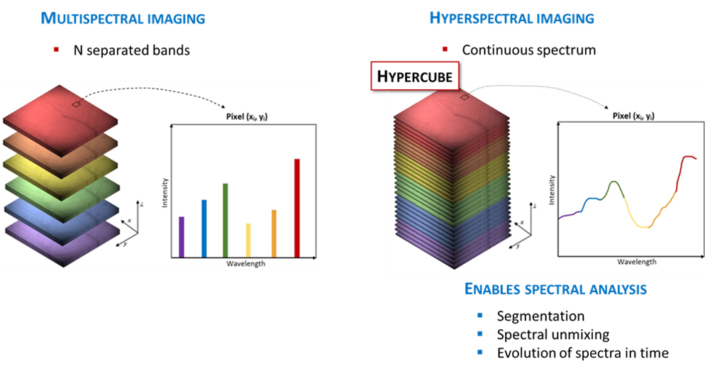
\includegraphics[width=0.7\linewidth]{media/images/hyperspectral_image.png}
    \caption{Esquemas para almacenar los valores de píxel reales de una imagen en un archivo \acrshort{bil}, referencia: \cite{Archivos82:online}}
    \label{fig:hyperspectral_image}
\end{figure}

\begin{code}[numbers=left]{title=Gráfico de velas de los outliers, label=code:plot-outliers}{Python}
def plots_outliers(outliers_df: pd.DataFrame, column=53):
    fig, axes = plt.subplots(ncols=2, figsize=(10, 5))
    sns.histplot(outliers_df[column], binwidth=1, ax=axes[0])
    sns.boxplot(outliers_df[column], ax=axes[1])
    fig.tight_layout()
    plt.show()
\end{code}

\begin{code}[numbers=left]{title=Detección de outliers utilizando \textit{zscore}, label=code:zscore}{Python}
...
    zscore = np.abs(stats.zscore(df))
    data_clean = df[(zscore < 3).all(axis=1)]
    df = data_clean
...
\end{code}

\begin{code}[numbers=left]{title=Gráfico de curvas de aprendizaje, label=code:plot-learning-curves}{Python}
def plots_balancing(df, df_balanced):
    fig, axis = plt.subplots(ncols=2, figsize=(10, 5))
    fig.suptitle(f'Balance of {src.utils.dev_config.OBJECTIVE_COLUMN}')
    axis[0].set_title(f'Before balancing {src.utils.dev_config.OBJECTIVE_COLUMN}')
    axis[1].set_title(f'After balancing {src.utils.dev_config.OBJECTIVE_COLUMN}')
    plot_balance(df, ax, 0)
    plot_balance(df_balanced, ax, 1)
    f.tight_layout()
    plt.show()
z

def plot_balance(df, axis, axis_number):
    return sns.histplot(df[src.utils.dev_config.OBJECTIVE_COLUMN], ax=axis[axis_number] if axis_number else axis)
\end{code}

\begin{code}[numbers=left]{title=Gráfico de comparación del balanceo, label=code:plots_balancing}{Python}
def plot_learning_curves(model, model_name, x, y):
    x_train, x_val, y_train, y_val = train_test_split(x, y, test_size=0.2)
    train_errors, val_errors = [], []
    
    for m in range(5, len(x_train)):
        model.fit(x_train[:m], y_train[:m])
        y_train_predict = model.predict(x_train[:m])
        y_val_predict = model.predict(x_val)
        train_errors.append(metrics.fbeta_score(y_train[:m], y_train_predict, beta=2))
        val_errors.append(metrics.fbeta_score(y_val, y_val_predict, beta=2))
        
    plt.title(f'{model_name} - Learning curves')
    plt.plot(np.sqrt(train_errors), "r-+", linewidth=2, label="train")
    plt.plot(np.sqrt(val_errors), "b-", linewidth=3, label="val")
    plt.xlabel("Training set size")
    plt.ylabel("f2 score")
    plt.legend(loc="best")
    plt.show()
\end{code}

% ---------------------------------------------------------- %
% 
\clearpage

% APPENDIX
% \subfile{sections/appendix}
% \clearpage

% SPECIAL TERMS
\printglossary[title=Definiciones adicionales, nonumberlist]\ \label{sec:additional-definitions}
\clearpage

% BIBLIOGRAPHY
\printbibliography[heading=bibintoc, title=Bibliografía y referencias]


\end{document}